\chapter{Tesztek laborkörülmények között}

\section{A kísérleti rendszer}
Az elméleti eredmények validálásához elkészítettük egy szoba kicsinyített modelljét. Ez egy kartondobozban kapott helyet. A doboz hőtároló képessége elég csekély, ezért extra hőtároló tömegeket helyeztünk a 
A fűtési teljesítményt halogén izzókkal juttattuk a rendszerbe. Ezek teljesítménye szabályozható, így ez a bemenet lineáris a szelepekkel ellentétben, azaz kétszer nagyobb beavatkozójelre kétszer nagyobb teljesítmény kerül a rendszerbe.
A hőmérsékletet mérjük a dobozban és azon kívül is. Zavarásként a mérőszoba ablakát kinyitjuk, így a doboz környezeti hőmérséklete lecsökken.

\section{A Simulink konfigurálása}
A real time futáshoz Simulink  Real-time szükséges. A real-time működés itt azt jelenti, hogy a szabályzót a Simulink mintavételi időnként futtatja le. Azaz ha a kísérleti rendszerre \SI{30}{\second}-es mintavételi idejű szabályzót tervezek, akkor az MPC félpercenként mintát fog venni a hőmérsékletekből és ki fog adni egy beavatkozójelet. Így a real-time ez esetben nem jelent például szigorú korlátokat a futásidőre.


%A Real-time UDP-t használom. %https://uk.mathworks.com/help/xpc/io_ref/udp-transport-protocol.html
%https://uk.mathworks.com/products/simulink-desktop-real-time.html

A szabályzó a számítógépen fog futni, és mintavételi időnként a jelenlegi hőmérsékletet beolvassa, az MPC-t lefuttatja, a beavatkozó jeleket pedig elküldi a beágyazott számítógépnek.

\begin{figure}
	\centering
	\begin{tikzpicture}[>=stealth,
  		%inner/.style={draw,fill=blue!5,thick,inner sep=3pt,minimum width=8em},
		%outer/.style={draw=gray,dashed,fill=green!1,thick,inner sep=5pt}
		outer/.style={draw=gray,dashed,thick,inner sep=5pt}
		]
	
	% Szabályzási kör elemei
	% ----------------------
	
		% Szabályzó
		\node[draw,rectangle, minimum height=2cm,minimum width=6cm] (MPC) at (3.2,3.5) {\parbox{2cm}{\centering MPC szabályozás}};		

		% Fűtési rendszer
		\node[draw,rectangle, minimum height=1.6cm,minimum width=5cm] (Heat) at (7,0) {\parbox{2cm}{\centering iContrALL~~~~ \\ dimmer~~}};
	
		% Ház
		\node[draw,rectangle, minimum height=1.6cm,minimum width=3.2cm] (House) at (2,0) {helyiség modellje};
		
		% Hőmérő
		\node[draw,rectangle, minimum height=1.6cm,minimum width=3.2cm] (Measure) at (-2,0) {\parbox{2cm}{\centering hőmérséklet\\mérés}};
		
		%Zavarás
		\node[rectangle, minimum height=0.8cm,minimum width=2cm,below=of House, node distance=1cm] (ghostDist)  {Zavarás};

		
	
	% Kiegészítő cuccok
	% ----------------------
	
	% Keret - Matlab
	\node[draw,outer,rectangle, minimum height=4cm,minimum width=8cm,
	label={[label distance=-0.1cm, anchor=north]100:Simulink, számítógépen real-time fut}] (keret) at (3.2,3.5) {};
	
	% Zavarás a modellbemenetre
	\draw[->] (ghostDist.90) --  (House.270) node[above]{$T_e$};
	
	%\draw[->] (ctr.191) node[right]{${u_{2}}$} -| ++(-1.7,1.3)|-  (Numeric.172) node[right]{$\alpha_{floor}$};  %node[above left]{$\alpha_{radiator}$}; 
	
	% mért változók
	\draw[->] (House.180) -- (Measure.0);
	\draw[->] (Measure.195) node[right]{$T_e$} -| ++(-1.2,0)  |-  (MPC.168) node[right]{MD} ;
	\draw[->] (Measure.165) node[right]{${T_{i}}$}-| ++(-0.5,0.8)  |-  (MPC.188) node[right]{MO} ;

	
	%\draw[->] (d.0) node[left]{heat [W]} ->  ++(3,0) ->  (house.180);
	% Beavatkozó jel
	\draw [->] (MPC.0) node[left]{MV} -| ++(4,-2.5)  |- (Heat.0) node[left]{${u_1}$}; %++(1.5cm,0) -- (2cm,0pt) -- (2.5cm,10pt);
	
	\draw[->] (Heat.180)  node[right]{$Q_{ki}$} -- (House.0) ;
	%\draw[->] (d.20) -| ++(1,-1) |- (y.350);
	
	%\path 
	%(d.150)	 edge[<->] 	node[anchor=north,above]{valvePercent}	(y.270);
	
	% Lehetséges label beállítások:
		%label={[blue,yshift=0.3cm]above:Z}]
	
%	\node[draw,outer,rectangle, minimum height=5.5cm,minimum width=13cm,
%	label={[label distance=-0.1cm, anchor=north]270:3 bemenetű, 1 kimenetű szakaszmodell}] (keret) at (0,15) {};
%	
%	
	\end{tikzpicture}

	\caption{A valós idejű mérések szereplői}
	\label{fig:realtimesimulink}
\end{figure}

%\begin{tikzpicture}[>=stealth,remember picture]
%\node[draw,rectangle,inner sep=0.5cm] (y) at (0,0) {$A$};
%\node[draw] (d) at (0,2) {%
%%	\begin{tikzpicture}[remember picture]
%%	\matrix [matrix of math nodes] (mat)
%%	{
%%		B & \phantom{C}   \\
%%		\phantom{B} & C \\
%%	};
%%	\end{tikzpicture}
%%};
%%\draw[->,shorten >= 6pt] (y.west) -| ++(-1,1) |- (mat-1-1);
%%\draw[->,shorten >= 6pt] (y.west) -| ++(-0.8,1) |- (mat-2-1);
%%\draw[->] ($(mat-2-2)+(14pt,0)$) -| ++(0.8,-1) |- (y.east);
%%\draw[->] ($(mat-1-2)+(14pt,0)$) -| ++(1,-1) |- (y.east);
%\end{tikzpicture}




% 3600001117-es ID-jű, Raspberry Pi, IP címe fixen 192.168.0.108, 54321-es port.

A PI SPI-n küld a rádióadónak.
Rádiókommunikáció egyirányú.

\section{Mintavételi idő és predikciós horizont}

Az MPC paraméterezésére \textit{Agachi \cite{romanMPC_Agachi}} könyvében találhatók ajánlások. A predikciós horizontot eszerint úgy kell megválasztani, hogy az a szakasz releváns dinamikáját lefedje. Mivel a felfutási ideje a kísérleti rendszernek kb. 1 óra, ezért ezt ekkorára választottam. A predikciós horizont ajánlott nagysága 10-20 mintavétel, a számítási igény csökkentése miatt. Ezért a mintavételi időt 300 másodpercnek (5 perc) vettem.

A fentiek mellett viszont a szabályzó nem adott ki beavatkozójelet egészen egy predikciós horizontnyi ideig, azaz majdnem 1 órán keresztül\footnote{Ha 30 másodperces mintavételi időt használtam és 100 mintányi predikciós horizontot, ugyanez volt a helyzet. Ez idő alatt az MPC valószínűleg az állapotbecslőjét inicializálja.}. Az MPC képes a költségfüggvényben figyelembe venni a predikciós horizonton belül a referenciajel jövőbeli változásait (ez a \textit{Signal Previewing}), ezt kipróbáltam annak érdekében, hogy ezt a \say{holtidőt} csökkentsem, ám ellentétes hatást értem el.

A Simulink blokk viszont támogatja az MPC-nek kezdeti érték megadását. A kezdeti érték nélküli MPC-t szimulációban futtattam, majd leolvastam annak belső állapotát.



\section{Szabályozótervezés az identifikált modellre}


\begin{figure}[H]
	\begin{subfigure}[t]{0.32\textwidth}
		\centering
		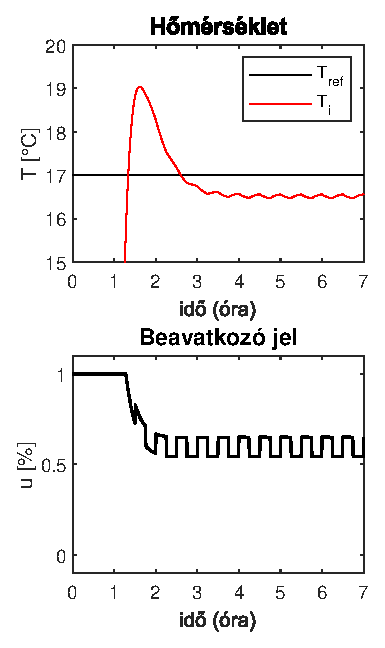
\includegraphics[width=\textwidth]{figures/realsys/mpc-wy-1}
		\caption{$y=1$ súly}
		\label{fig:mpc-wy-1}
	\end{subfigure}
	~
	\begin{subfigure}[t]{0.32\textwidth}
		\centering
		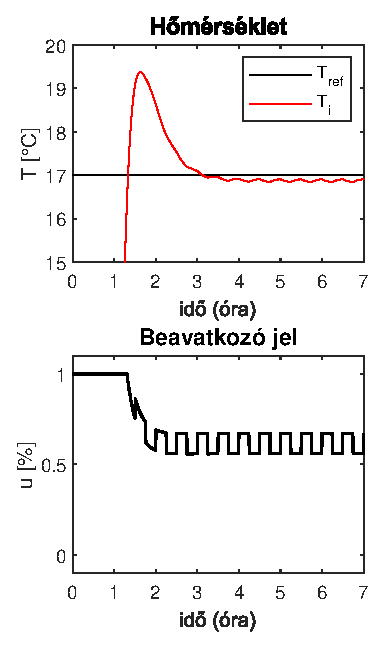
\includegraphics[width=\textwidth]{figures/realsys/mpc-wy-2}
		\caption{$y=2$ súly}
		\label{fig:mpc-wy-2}
	\end{subfigure}
	~
	\begin{subfigure}[t]{0.32\textwidth}
		\centering
		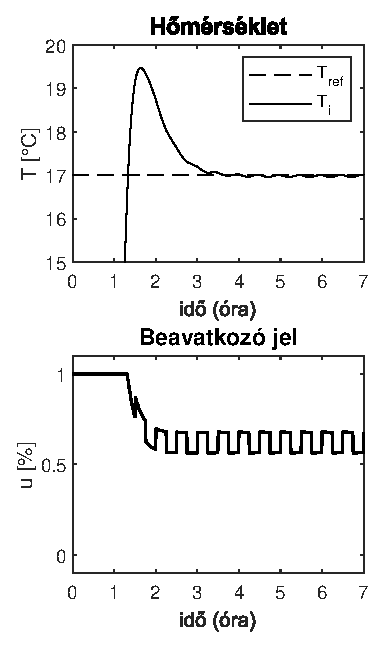
\includegraphics[width=\textwidth]{figures/realsys/mpc-wy-5}
		\caption{$y=5$ súly}
		\label{fig:mpc-wy-5}
	\end{subfigure}	
\end{figure}